% =====================================================================
% THIS FILE IS THE SOURCE. Edit it, then rebuild the PDF with:
%     bash tools/compile.sh Unit_11_Categorical_Outcomes
% (run from the Course_Rewrite folder; it compiles twice and reports
%  page count, overfull boxes, and em dashes)
%
% Do not edit the PDF directly. Figures are the fig_*.pdf files in this
% folder, regenerated by tools/make_module*_slide_figs.py.
%
% Originally converted from the 15-module draft by a one-shot script now
% parked in tools/one_shot_generators/. Re-running those would discard
% anything you change here, so they are kept out of tools/ on purpose.
% =====================================================================
\documentclass[aspectratio=169]{beamer}
\usetheme{default}
\usefonttheme{professionalfonts}
\usepackage{amsmath, amssymb, amsfonts}
\usepackage{graphicx}
\usepackage{booktabs}
\usepackage{bm}
\usepackage{hyperref}

\mode<presentation> {
    \usetheme{Frankfurt}
    \usecolortheme{default}
}

\newcommand{\xbar}{\bar{x}}
\newcommand{\yhat}{\hat{y}}
\newcommand{\PR}[1]{P(#1)}
\newcommand{\phat}{\hat{p}}

\newenvironment{principle}[1]{\begin{block}{\textbf{Principle:} #1}}{\end{block}}
\newenvironment{trap}[1]{\begin{alertblock}{\textbf{Trap:} #1}}{\end{alertblock}}
\newenvironment{practice}[1]{\begin{exampleblock}{\textbf{In practice:} #1}}{\end{exampleblock}}
\newenvironment{interview}[1]{\begin{exampleblock}{\textbf{You may be asked:} #1}}{\end{exampleblock}}
\newenvironment{yourturn}[1]{%
  \setbeamercolor{block title}{fg=white,bg=orange!80!black}%
  \setbeamercolor{block body}{bg=orange!12}%
  \begin{block}{\textbf{Your turn:} #1}}{\end{block}}
\newenvironment{livedemo}[1]{%
  \setbeamercolor{block title}{fg=white,bg=teal!80!black}%
  \setbeamercolor{block body}{bg=teal!12}%
  \begin{block}{\textbf{Live demo:} #1}}{\end{block}}
\newenvironment{llmcheck}[1]{%
  \setbeamercolor{block title}{fg=white,bg=violet!75!black}%
  \setbeamercolor{block body}{bg=violet!10}%
  \begin{block}{\textbf{LLM check:} #1}}{\end{block}}

\title{Categorical Outcomes}
\subtitle{Unit 11: Rates, Tables, and Predicting a Yes or No}
\author{Stat 220 \textbar{} Statistics for Data Science}
\date{}

\begin{document}

\begin{frame}
  \titlepage
\end{frame}

% ======================================================================
\section{Proportions}
% ======================================================================
\begin{frame}{Where this fits}
\begin{itemize}
  \item Part I predicted \emph{numbers}. An enormous share of real data is not a number: converted
        or not, churned or not, fraud or not, which region, which plan.
  \item This unit needed Part II first. Odds, base rates, and predictive values are conditional
        probability wearing different hats, and we only built that in Unit 7.
  \item Three arcs: describing rates honestly, comparing them in tables, and modeling a yes or no
        and turning it into a decision.
\end{itemize}
\begin{principle}{a rate is a fraction with a story on both floors}
Every rate has a numerator and a denominator, and most arguments about rates are really arguments
about the denominator.
\end{principle}
\end{frame}

\begin{frame}{Live experiment: the rock-paper-scissors tournament}
\begin{livedemo}{can you be random?}
Pair up. Play \textbf{five rounds} of rock-paper-scissors. One person in each pair records
\emph{only the first throw} of each round for both players.
\begin{itemize}
  \item We will collect every first throw on the board as three counts.
  \item Then we test the hypothesis everyone assumes: that people throw each option one third of
        the time.
\end{itemize}
\end{livedemo}
\vspace{0.2em}
{\tiny\textit{Materials: none. Time: 8 minutes including tallying the throws.}}
\centering\small Winners of the most rounds, keep your hand up. We will come back to whether you
were lucky or good.
\end{frame}
\begin{frame}{Stay here while they play: what the research says}
\begin{columns}[c]
\begin{column}{0.55\textwidth}
\centering
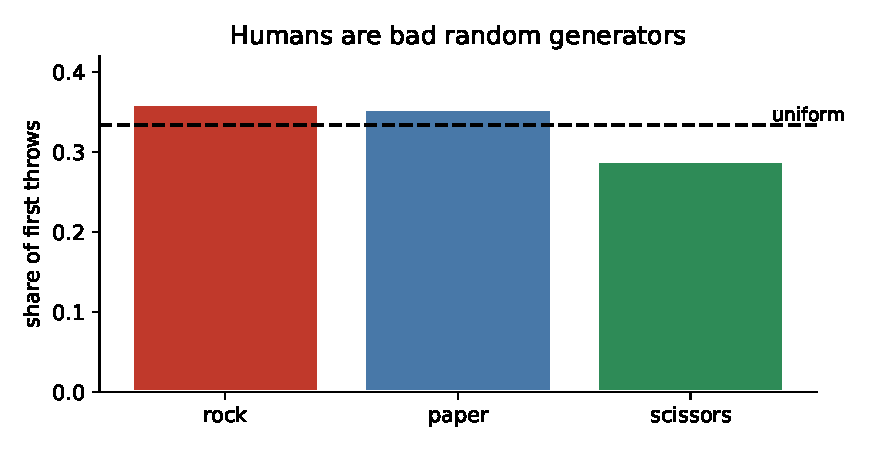
\includegraphics[width=\textwidth]{fig_m10_rps.pdf}
\end{column}
\begin{column}{0.45\textwidth}
\small
Across large studies of first throws:
\begin{itemize}
  \item \textbf{Rock} is thrown about 36\% of the time, scissors only about 29\%.
  \item So ``always play paper'' beats a typical human opponent slightly more often than it loses.
\end{itemize}
The edge is small, but it is free, and it exists because people cannot generate randomness.
\end{column}
\end{columns}
\end{frame}
\begin{frame}{Testing our own counts}
Suppose the class produced $n$ throws with counts $O_{\text{rock}}, O_{\text{paper}},
O_{\text{scissors}}$. Under ``all equally likely,'' each expected count is $E = n/3$.
\[
\chi^2 = \sum \frac{(O - E)^2}{E}, \qquad \text{compare to a chi-square with 2 degrees of freedom.}
\]
\begin{itemize}
  \item Bigger than about \textbf{6} means the pattern is hard to explain by chance.
  \item This is the same signal-to-noise logic as always: how far are the observed counts from
        what the null predicts, measured in units of how far they normally wander?
\end{itemize}
\end{frame}
\begin{frame}{What this unit gives you}
\begin{columns}[T]
\begin{column}{0.5\textwidth}
\textbf{Things to know}
\begin{itemize}\small
  \item how to estimate a proportion and put an honest interval on it
  \item the three ways to express a comparison, and how differently they read
  \item contingency tables and chi-square, and what they do \emph{not} say
  \item why denominators and group mix can reverse a conclusion
  \item logistic regression, log-odds, and odds ratios
  \item precision, recall, ROC/AUC, thresholds, and calibration
\end{itemize}
\end{column}
\begin{column}{0.5\textwidth}
\textbf{Mistakes to stop making}
\begin{itemize}\small
  \item quoting a relative change with no base rate
  \item confusing percentage points with percent
  \item reading a significant chi-square as a large or causal effect
  \item pooling across a variable that drives the outcome
  \item reporting accuracy on imbalanced data
  \item leaving the threshold at 0.5 because it is the default
\end{itemize}
\end{column}
\end{columns}
\end{frame}

\begin{frame}{One proportion, with honest uncertainty}
\[
\phat = \frac{x}{n}, \qquad \mathrm{SE}(\phat) = \sqrt{\frac{\phat(1-\phat)}{n}},
\qquad \phat \pm 1.96\,\mathrm{SE}.
\]
\begin{itemize}
  \item 12 conversions out of 300: $\phat = 0.04$, SE $= 0.011$, interval roughly 1.8\% to 6.2\%.
  \item That is a \emph{wide} interval, and reporting ``our conversion rate is 4\%'' hides it
        completely.
\end{itemize}
\begin{principle}{a percentage is an estimate too}
Every rate you have ever seen on a dashboard has a standard error. Most dashboards do not show it,
and most arguments about week-over-week movement are arguments about noise.
\end{principle}
\end{frame}
\begin{frame}{When the count is small, patch the interval}
\begin{itemize}
  \item With few successes the standard formula misbehaves badly. Zero successes gives
        $\mathrm{SE} = 0$ and an interval of zero width, which is obviously wrong.
  \item Simple fix (the \textbf{plus-four} interval): add 2 successes and 2 failures, then use the
        usual formula. It works remarkably well.
  \item Zero out of 20 does not mean ``never.'' A useful rough bound: with 0 events in $n$ trials,
        the rate could plausibly be as high as $3/n$.
\end{itemize}
\begin{practice}{a question that catches people}
``We saw no failures in 50 tests. What is our failure rate?'' The good answer: ``Not zero. The
data is consistent with anything up to about 6\%.''
\end{practice}
\end{frame}
\begin{frame}{Comparing two proportions: three languages}
A campaign moves conversion from 2.0\% to 2.4\%.
\begin{itemize}
  \item \textbf{Absolute difference:} $+0.4$ \emph{percentage points}.
  \item \textbf{Relative difference:} $+20\%$ (a fifth more).
  \item \textbf{Odds ratio:} about 1.21.
\end{itemize}
All three are true. They will produce three different meetings.
\begin{trap}{percent versus percentage points}
Going from 2\% to 2.4\% is a rise of 0.4 percentage points \emph{or} 20 percent. Writing ``a 20\%
increase'' when you meant 0.4 points, or the reverse, is the single most common numerical error in
business writing.
\end{trap}
\end{frame}
\begin{frame}{Relative risk without a base rate is not usable}
\begin{center}
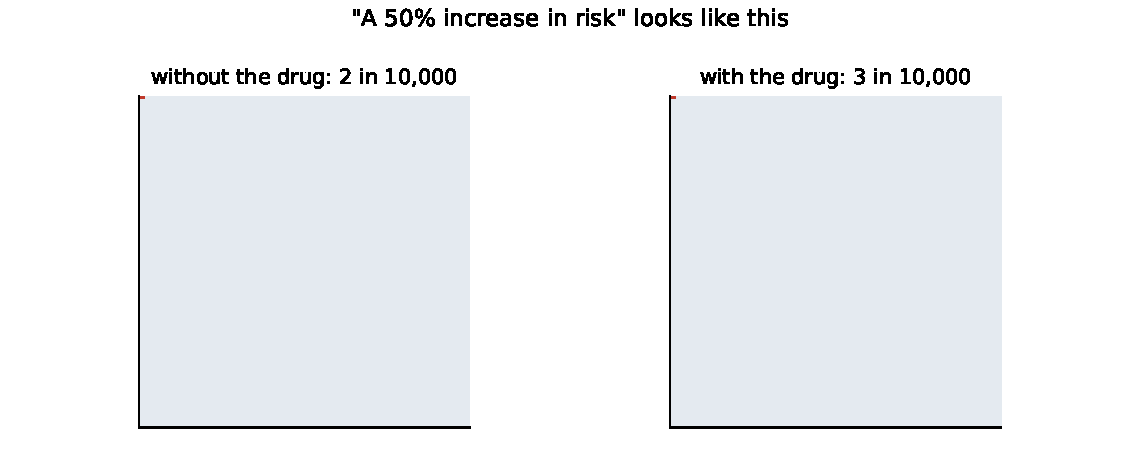
\includegraphics[width=0.86\textwidth]{fig_m10_relrisk.pdf}
\end{center}
\vspace{-0.4em}
\small
``This drug increases your risk by 50\%'' describes the move from 2 in 10{,}000 to 3 in 10{,}000.
Both squares look empty because both risks are tiny. The headline is accurate and useless.
\end{frame}
\begin{frame}{Your turn \#1}
\begin{yourturn}{translate the headline}
A news story reports: ``Eating processed meat daily raises your risk of colorectal cancer by
18\%.'' The lifetime risk without it is about 5\%.
\vspace{0.3em}

With a neighbor: what is the risk \emph{with} daily processed meat, in absolute terms? How would
you write the headline honestly, and would you change your diet?
\end{yourturn}
\end{frame}
\begin{frame}{Your turn \#1: answer}
\begin{itemize}
  \item A relative increase of 18\% on a 5\% baseline gives about \textbf{5.9\%}: roughly one extra
        case per 100 people.
  \item Honest version: ``about 5 in 100 people get colorectal cancer, and among daily processed-meat
        eaters it is about 6 in 100.''
  \item Whether to change your diet is now a real decision with real numbers, instead of a reaction
        to the word ``raises.''
\end{itemize}
\begin{principle}{always report both}
Give the relative change \emph{and} the absolute change. One without the other is a choice about
how alarmed you want your audience to be.
\end{principle}
\end{frame}
% ======================================================================
\section{Tables and models}
% ======================================================================
\begin{frame}{The contingency table}
Cross-tabulate two categorical variables and ask whether they are related.
\begin{itemize}
  \item \textbf{Null hypothesis:} the two variables are independent, so the row percentages should
        be the same in every row.
  \item \textbf{Expected count} for a cell: $\dfrac{(\text{row total})(\text{column total})}
        {\text{grand total}}$, which is exactly what independence implies.
  \item \textbf{Chi-square} adds up $(O - E)^2/E$ over all cells, with
        $(\text{rows}-1)(\text{columns}-1)$ degrees of freedom.
\end{itemize}
\end{frame}
\begin{frame}{A real table: loan purpose and default}
\begin{columns}[c]
\begin{column}{0.6\textwidth}
\centering
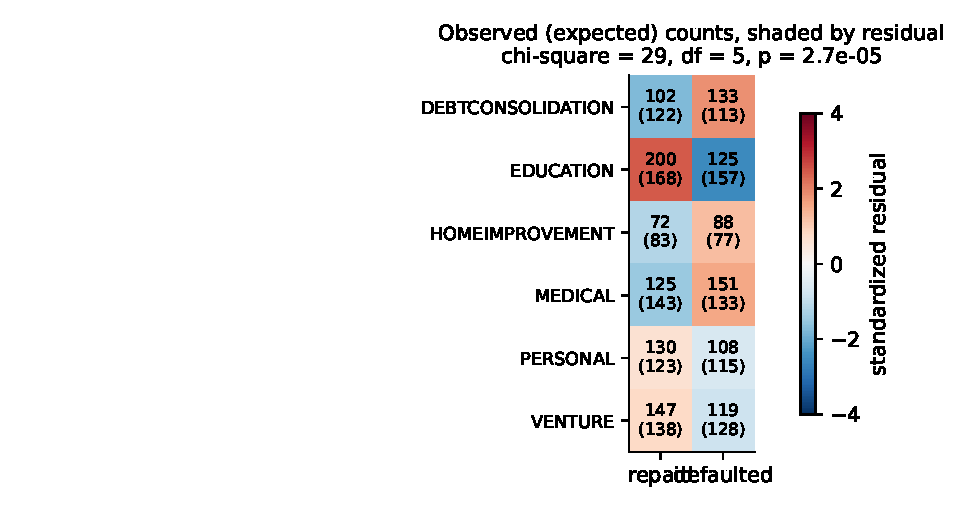
\includegraphics[width=\textwidth]{fig_m10_chisq.pdf}
\end{column}
\begin{column}{0.4\textwidth}
\small
1{,}500 consumer loans.
\begin{itemize}
  \item Education loans default far less than expected. Debt consolidation and medical loans default far
        more.
  \item The test says the association is real ($p \approx 3 \times 10^{-5}$).
  \item It does \emph{not} say the purpose causes the default, or how large the effect is.
\end{itemize}
\end{column}
\end{columns}
\end{frame}
\begin{frame}{What a chi-square test does not tell you}
\begin{itemize}
  \item \textbf{Not the size} of the association. With 100{,}000 rows, a trivial dependence
        produces an enormous chi-square.
  \item \textbf{Not the direction or the pattern.} Follow up with the residuals to see which cells
        drive it, as in the figure.
  \item \textbf{Not causation.} It is an association in observational data, subject to every
        confounder you have not measured.
\end{itemize}
\begin{trap}{significance is not strength}
Report the actual rates alongside the test. ``Education loans default at 38\% versus 57\% for debt
consolidation'' is informative. ``$p < 0.001$'' by itself is not.
\end{trap}
\end{frame}
\begin{frame}{Assumptions and the small-cell problem}
\begin{itemize}
  \item The chi-square approximation needs reasonably large \textbf{expected} counts, roughly 5 or
        more in most cells.
  \item With sparse tables, use Fisher's exact test or combine categories that belong together.
  \item Every observation must be an independent unit. A table built from repeated measurements on
        the same customers overstates the evidence dramatically.
\end{itemize}
\begin{trap}{the cell-hunting expedition}
A 6-by-4 table has 24 cells. Scanning them for the ``significant'' one is 24 tests, and something
will always look striking. Decide what you are testing before you look.
\end{trap}
\end{frame}
\begin{frame}{Counts mislead. Rates need the right denominator}
\begin{itemize}
  \item ``Region A had 340 complaints, Region B had 120.'' Region A also has four times the
        customers.
  \item The denominator should be the \textbf{exposure}: customers, shipments, patient-days, miles
        driven, hours of use.
  \item Choosing the denominator is a modeling decision. Accidents per driver, per mile, and per
        trip can rank the same drivers differently.
\end{itemize}
\begin{practice}{a good instinct to show}
``Before I compare those numbers I want to know what each one is divided by, and whether the two
denominators mean the same thing.''
\end{practice}
\end{frame}
\begin{frame}{Standardization: comparing apples to apples}
\begin{itemize}
  \item Hospital A has a higher death rate than Hospital B. Hospital A is a trauma center that
        receives the sickest patients.
  \item The fix is \textbf{standardization}: compute the rate within each risk group, then combine
        using a common population mix.
  \item This is how age-adjusted mortality rates, risk-adjusted surgical outcomes, and
        seasonally-adjusted economic figures are built.
\end{itemize}
\begin{principle}{adjust before you rank}
Any ranking of units that serve different populations is a ranking of the populations until you
adjust for the mix.
\end{principle}
\end{frame}
\begin{frame}{Simpson's paradox, with the famous real case}
\begin{center}
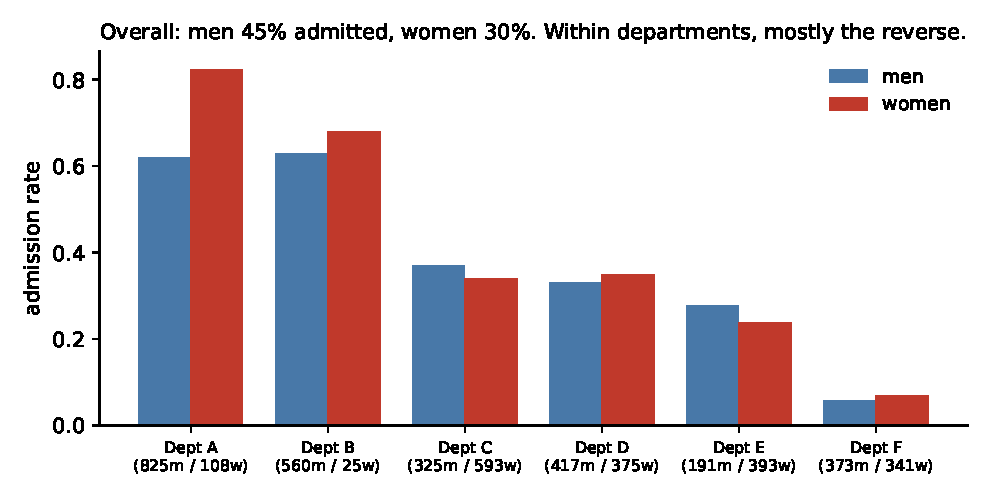
\includegraphics[width=0.83\textwidth]{fig_m10_simpson.pdf}
\end{center}
\vspace{-0.5em}
\small
Berkeley graduate admissions, 1973. Overall, 44\% of men and 30\% of women were admitted, and the
university was sued. Department by department, women fared similarly or better. The difference:
women applied far more often to the departments that admitted almost nobody.
\end{frame}
\begin{frame}{Why the reversal happens, and what to do}
\begin{itemize}
  \item Aggregating mixes together groups with very different base rates and very different sizes.
        The pooled number is a weighted average with the wrong weights.
  \item The paradox appears whenever a \textbf{lurking variable} (here, department) affects both
        the group assignment and the outcome.
  \item The remedy is to \emph{disaggregate}, or to model the outcome with the lurking variable
        included, exactly as you learned to do with a confounder in regression.
\end{itemize}
\begin{trap}{the aggregated conclusion}
Any single number computed across heterogeneous groups can be reversed by regrouping. Before you
present one, ask what happens within the obvious subgroups.
\end{trap}
\end{frame}
\begin{frame}{Your turn \#2}
\begin{yourturn}{find the lurking variable}
A hospital reports that patients treated by Surgeon X have a 12\% complication rate, versus 6\%
for Surgeon Y. Administration proposes retraining Surgeon X.
\vspace{0.3em}

With a neighbor: name two variables that could reverse this comparison, and state what you would
compute instead.
\end{yourturn}
\end{frame}
\begin{frame}{Your turn \#2: answer}
\begin{itemize}
  \item \textbf{Case severity} is the obvious one: the best surgeon often gets the hardest cases,
        which guarantees a worse raw rate.
  \item \textbf{Volume and case mix}: emergency versus scheduled, patient age, comorbidities.
  \item What to compute: complication rates \emph{within} severity strata, or a model that adjusts
        for the risk factors, plus intervals so you can see whether 12\% and 6\% are even
        distinguishable given the number of operations.
\end{itemize}
\begin{principle}{the referral pattern is part of the data}
Whenever units receive different inputs, the raw output comparison measures the inputs.
\end{principle}
\end{frame}
\begin{frame}{Why not just fit a line?}
\begin{itemize}
  \item If $y$ is 0 or 1, a straight line predicts probabilities above 1 and below 0, which is
        nonsense.
  \item Logistic regression fits a line on the \textbf{log-odds} scale and then bends it into the
        0-to-1 range:
\end{itemize}
\[
\log\frac{p}{1-p} = b_0 + b_1x_1 + \cdots + b_kx_k
\qquad\Longleftrightarrow\qquad
p = \frac{1}{1 + e^{-(b_0 + b_1x_1 + \cdots)}}
\]
\begin{principle}{same skeleton as regression}
Predictors combine linearly, coefficients come with standard errors, and the estimate-over-SE
template still tells you what is real. Only the link to the outcome changed.
\end{principle}
\end{frame}
\begin{frame}{The curve, on real patient data}
\begin{columns}[c]
\begin{column}{0.58\textwidth}
\centering
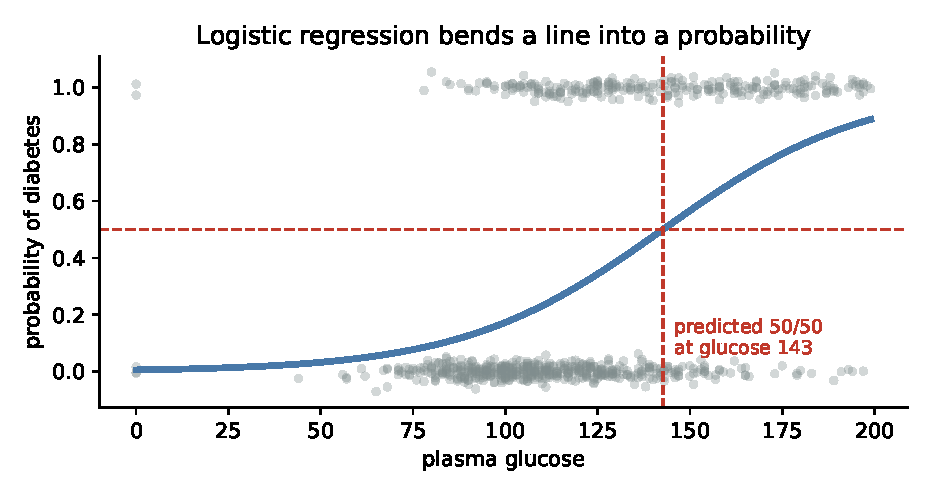
\includegraphics[width=\textwidth]{fig_m09_logistic.pdf}
\end{column}
\begin{column}{0.42\textwidth}
\small
733 patients, predicting a diabetes diagnosis from plasma glucose.
\begin{itemize}
  \item Each dot is a person at 0 or 1 (jittered so you can see them).
  \item The curve is the fitted probability. It is steep in the middle and flat at the ends, which
        is exactly how evidence should work.
\end{itemize}
\end{column}
\end{columns}
\end{frame}
\begin{frame}{Reading a logistic coefficient out loud}
\begin{itemize}
  \item A coefficient $b_1$ is a change in \textbf{log-odds} per unit of $x$. Nobody thinks in
        log-odds.
  \item Exponentiate it: $e^{b_1}$ is an \textbf{odds ratio}. If $e^{b_1} = 1.35$, each extra unit
        multiplies the odds by 1.35, a 35\% increase in the odds.
  \item Rough translation for small effects: divide the coefficient by 4 to get the maximum change
        in probability per unit.
\end{itemize}
\begin{trap}{odds are not probabilities}
``The odds tripled'' does not mean ``three times as likely'' in probability terms. Going from 1\%
to 3\% and from 30\% to 56\% are both a tripling of odds, and they feel completely different to
the business.
\end{trap}
\end{frame}
% ======================================================================
\section{Decisions}
% ======================================================================
\begin{frame}{Live experiment: the inbox game}
\begin{livedemo}{you are the spam filter}
Each team gets the same list of 20 emails, with the model's spam score for each (0 to 1) and a
short description. Your job: pick \textbf{one threshold}. Everything at or above it goes to the
spam folder.
\begin{itemize}
  \item Missing a spam email (it lands in the inbox): costs you \textbf{1 point}.
  \item Blocking a real email (a job offer in the spam folder): costs you \textbf{10 points}.
\end{itemize}
Write your threshold on the board. Lowest total cost wins.
\end{livedemo}
\vspace{0.2em}
{\tiny\textit{Materials: the email table on the next slide. Time: 10 minutes.}}
\centering\small Do not compute anything yet. Pick the number your gut says, then we will score it.
\end{frame}
\begin{frame}{The inbox: 20 emails and the model's spam score}
\begin{columns}[T]
\begin{column}{0.5\textwidth}
\scriptsize
\begin{tabular}{@{}ll@{}}
\toprule
score & subject \\
\midrule
0.97 & Nigerian prince, urgent transfer \\
0.95 & FREE CRYPTO GIVEAWAY!!! \\
0.93 & Refinance now, rates expire \\
0.91 & Recruiter: internship at Adobe \\
0.88 & You have won a gift card \\
0.84 & Weight loss miracle \\
0.79 & Career fair: employers attending \\
0.74 & Invoice attached, unknown vendor \\
0.68 & Professor: exam rescheduled \\
0.61 & Limited time software offer \\
\bottomrule
\end{tabular}
\end{column}
\begin{column}{0.5\textwidth}
\scriptsize
\begin{tabular}{@{}ll@{}}
\toprule
score & subject \\
\midrule
0.55 & Bank: unusual sign-in detected \\
0.49 & Newsletter you never wanted \\
0.44 & Landlord: lease renewal \\
0.38 & Group project meeting Thursday \\
0.31 & Conference invite, pay to publish \\
0.26 & Airline: flight delayed \\
0.19 & Mom: call me \\
0.13 & GitHub: pull request review \\
0.08 & Bill due Friday \\
0.03 & Slack digest \\
\bottomrule
\end{tabular}
\end{column}
\end{columns}
\vspace{0.4em}
\centering\small
One threshold per team. Miss a spam: 1 point. Block a real email: 10 points.
\end{frame}
\begin{frame}{Stay here while they choose: what will happen}
\begin{itemize}
  \item Teams that picked \textbf{0.5} because it is the default will do poorly.
  \item Because blocking real mail is ten times worse, the winning threshold will be high,
        somewhere around \textbf{0.9}: only block when you are very sure.
  \item Now flip the costs. If we were filtering \emph{phishing attacks in a hospital}, missing
        one is catastrophic and the threshold should be low.
\end{itemize}
\end{frame}
\begin{frame}{Scoring the inbox game}
\centering
\small
\begin{tabular}{@{}lccc@{}}
\toprule
threshold & real emails blocked & spam missed & \textbf{total cost} \\
\midrule
0.30 & 6 & 0 & 60 \\
0.50 (the default) & 4 & 2 & \textbf{42} \\
0.70 & 2 & 3 & 23 \\
0.80 & 1 & 4 & 14 \\
\textbf{0.92} & \textbf{0} & \textbf{6} & \textbf{6} \\
1.00 (block nothing) & 0 & 9 & 9 \\
\bottomrule
\end{tabular}
\vspace{0.5em}

\onslide<2->{%
\begin{principle}{the threshold is a business decision, not a modeling one}
The best threshold here is \textbf{0.92}, seven times cheaper than the 0.5 default. The model never
changed. Only the number you compared it to did, and that number came from the \emph{costs}, not
from the data.
\end{principle}}
\end{frame}
\begin{frame}{The confusion matrix, and the two ways to be wrong}
\begin{itemize}
  \item \textbf{True positive:} you said yes and it was yes.
  \item \textbf{False positive:} you said yes and it was no. A false alarm.
  \item \textbf{False negative:} you said no and it was yes. A miss.
  \item \textbf{True negative:} you said no and it was no.
\end{itemize}
\[
\text{precision} = \frac{TP}{TP + FP} \quad\text{(of those I flagged, how many were real?)}
\]
\[
\text{recall} = \frac{TP}{TP + FN} \quad\text{(of the real ones, how many did I catch?)}
\]
\end{frame}
\begin{frame}{Two thresholds on the same model}
\begin{center}
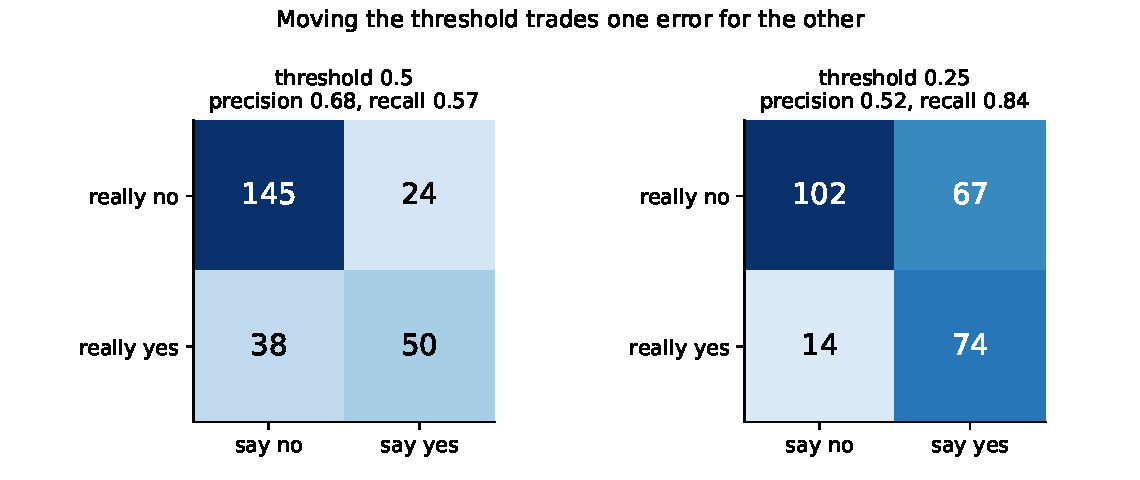
\includegraphics[width=0.9\textwidth]{fig_m09_confusion.pdf}
\end{center}
\vspace{-0.4em}
\small
Same model, same test set, one number changed. Lowering the threshold from 0.5 to 0.25 catches
many more real cases (recall rises) at the price of more false alarms (precision falls). No
\emph{threshold} improves both at once. Only a better model does, which is why the threshold and
the model are separate decisions.
\end{frame}
\begin{frame}{Which one do you care about?}
\begin{itemize}
  \item \textbf{Recall matters most} when a miss is catastrophic: cancer screening, fraud on a
        large account, safety alerts.
  \item \textbf{Precision matters most} when acting is expensive or annoying: sending a technician,
        blocking a customer's card, flooding a review queue.
  \item Almost every real system needs a stated tradeoff, not a single metric.
\end{itemize}
\begin{interview}{answer this way}
``It depends on the cost of each error. If missing a fraudulent charge costs \$400 and reviewing a
false alarm costs \$3, I want recall, and I would set the threshold from that ratio.''
\end{interview}
\end{frame}
\begin{frame}{Why accuracy lies}
\begin{itemize}
  \item In our test set, 34\% of patients have diabetes. A model that predicts ``no'' for everyone
        scores \textbf{66\% accuracy} and is worthless.
  \item Make the disease rarer, say 1 in 1000, and ``always no'' scores \textbf{99.9\%}.
  \item Accuracy rewards predicting the majority class, which is exactly what you do not need a
        model for.
\end{itemize}
\begin{trap}{the interview trap you will definitely be asked}
``Our model is 99\% accurate.'' The correct first question is always: \emph{what is the base rate,
and what does the trivial model score?}
\end{trap}
\end{frame}
\begin{frame}{ROC and precision-recall curves}
\begin{center}
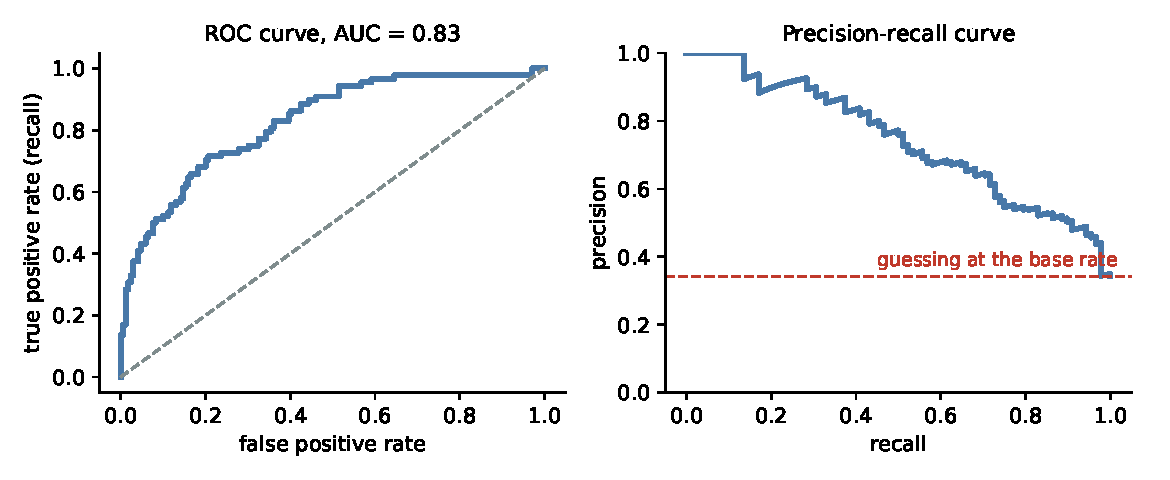
\includegraphics[width=0.9\textwidth]{fig_m09_roc.pdf}
\end{center}
\vspace{-0.4em}
\small
The ROC curve sweeps every threshold at once, and AUC is the area under it (0.83 here). AUC is the
chance the model ranks a random positive above a random negative. On imbalanced problems the
precision-recall curve is far more informative, because it shows what fraction of your flagged
queue is real.
\end{frame}
\begin{frame}{What AUC does and does not tell you}
\begin{itemize}
  \item \textbf{Does:} summarize ranking quality across all thresholds, independent of the base
        rate. Good for comparing two models.
  \item \textbf{Does not:} tell you whether the model is useful, what threshold to use, whether
        the probabilities are honest, or whether the flagged queue is workable.
  \item A model with AUC 0.95 can still produce a queue that is 90\% false positives if the event
        is rare enough.
\end{itemize}
\begin{principle}{report the operating point, not just the curve}
``AUC 0.87'' is a modeling statistic. ``At our threshold we catch 62\% of fraud and 1 in 5 flags is
real'' is an answer someone can act on.
\end{principle}
\end{frame}
\begin{frame}{The threshold follows from the costs}
\begin{columns}[c]
\begin{column}{0.58\textwidth}
\centering
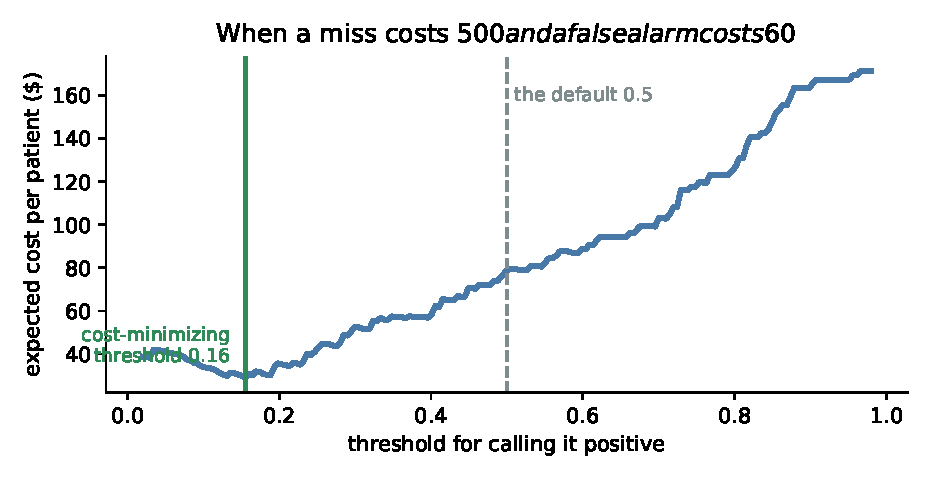
\includegraphics[width=\textwidth]{fig_m09_threshold.pdf}
\end{column}
\begin{column}{0.42\textwidth}
\small
Missing a case costs \$500 and an unnecessary follow-up costs \$60.
\begin{itemize}
  \item The cost-minimizing threshold is about \textbf{0.16}, not 0.5.
  \item Using the default would nearly double the expected cost per patient.
\end{itemize}
\end{column}
\end{columns}
\onslide<2->{\centering\small
Rule of thumb: the optimal threshold is near
$\text{cost}_{FP} / (\text{cost}_{FP} + \text{cost}_{FN})$.}
\end{frame}
\begin{frame}{Where 0.5 comes from, and why it is usually wrong}
\begin{itemize}
  \item 0.5 is optimal only when the two errors cost exactly the same. That is almost never true.
  \item It is a software default, not a decision. Every serious deployment tunes it.
  \item Tune it on \textbf{held-out} data, using real costs, and re-tune when the costs or the
        base rate change.
\end{itemize}
\begin{interview}{a question that separates candidates}
``Where would you set the threshold?'' A weak answer names a number. A strong answer asks for the
two costs and the base rate first, then names a number.
\end{interview}
\end{frame}
\begin{frame}{Class imbalance, handled honestly}
\begin{itemize}
  \item Imbalance is a fact about the world, not a modeling bug. Fraud really is rare.
  \item Reasonable responses: use precision-recall rather than accuracy, tune the threshold, weight
        the classes in the loss, or gather more positives.
  \item Resampling (oversampling positives, undersampling negatives) can help the fit, but it
        \textbf{distorts the predicted probabilities}. If you resample, you must recalibrate before
        anyone reads a probability.
\end{itemize}
\begin{trap}{the balanced-data trap}
A model trained on a 50/50 rebalanced sample will predict roughly 50\% probabilities in a world
where the true rate is 1\%. It ranks fine and its probabilities are fiction.
\end{trap}
\end{frame}
\begin{frame}{Calibration: does 30\% mean 30\%?}
\begin{columns}[c]
\begin{column}{0.54\textwidth}
\centering
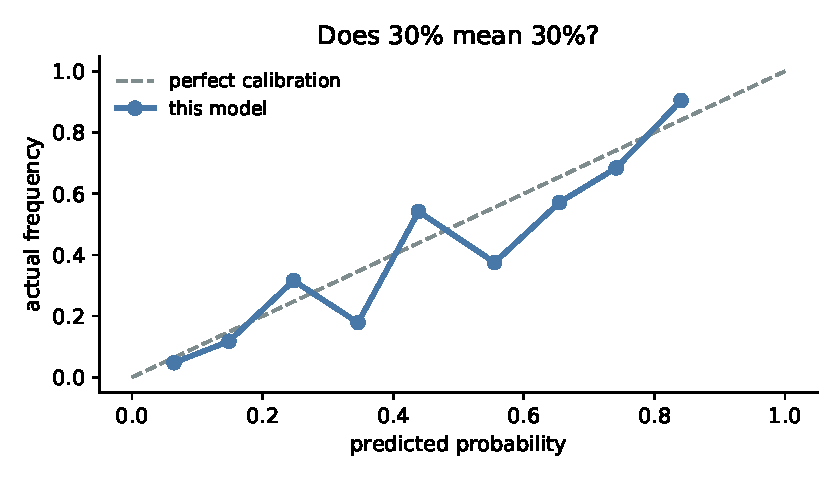
\includegraphics[width=\textwidth]{fig_m09_calibration.pdf}
\end{column}
\begin{column}{0.46\textwidth}
\small
Group the predictions into bins and check: among cases predicted at 30\%, did about 30\% actually
happen?
\begin{itemize}
  \item On the diagonal: calibrated, and the number can be used in an expected-value calculation.
  \item Off the diagonal: the ranking may still be fine, but the probabilities cannot be multiplied
        by dollars.
\end{itemize}
\end{column}
\end{columns}
\end{frame}
\begin{frame}{Your turn \#3}
\begin{yourturn}{set the threshold, defend it}
You build a model to flag transactions for manual review. Reviewing one costs \$4 of analyst time.
A missed fraud costs an average of \$220. Fraud is 0.3\% of transactions.
\vspace{0.3em}

With a neighbor: roughly where should the threshold go, and what is the one thing you must check
about the model before that number means anything?
\end{yourturn}
\end{frame}
\begin{frame}{Your turn \#3: answer}
\begin{itemize}
  \item The cost ratio gives a threshold around $4/(4 + 220) \approx \textbf{0.018}$. You review
        anything above roughly a 2\% chance of fraud.
  \item Most of that queue will be honest transactions, and that is correct: it is worth four
        dollars to avoid a one-in-fifty chance of losing \$220.
  \item The thing to check first: \textbf{calibration}. A threshold in probability units is
        meaningless if the model's ``2\%'' is not really 2\%.
\end{itemize}
\begin{principle}{expected value, one transaction at a time}
Flag when $\PR{\text{fraud}} \times \text{cost of a miss} > \text{cost of a review}$. Every
threshold decision is that comparison.
\end{principle}
\end{frame}
\begin{frame}{Scenario: the model that was too good}
\textbf{Setup.} A hospital model predicts which patients will be readmitted, with AUC 0.99 in
testing. In production it is useless.
\begin{itemize}
  \item Suspect \textbf{leakage} first. Something in the training data encoded the answer: a
        discharge code entered after readmission, or a billing field only filled in later.
  \item Check the timing of every feature: was this value knowable \emph{at the moment of
        prediction}?
  \item The AUC itself was the warning. Real clinical prediction lands around 0.7 to 0.85.
\end{itemize}
\begin{trap}{amazing performance is a symptom}
Your first reaction to a near-perfect classifier should be to hunt for leakage, not to celebrate.
\end{trap}
\end{frame}
% ======================================================================
\section{LLM check}
% ======================================================================
\begin{frame}{LLM check: mistake or not? (1 of 2)}
\begin{llmcheck}{we asked an LLM to interpret an A/B test}
\textbf{We told it:} ``Version A converted 20 of 500 visitors, version B converted 28 of 500. Is B
better?''\\[4pt]
\textbf{It answered:} ``Yes. B's conversion rate is 5.6\% versus A's 4.0\%, a 40\% improvement.
That is a substantial lift and you should roll out version B.''
\end{llmcheck}
\vspace{0.2em}
\centering\small Mistake, or no mistake?
\onslide<2->{%
\begin{trap}{verdict: mistake}
The difference is 1.6 percentage points with standard errors near 1 point each. A two-proportion
test gives $p \approx 0.25$: entirely consistent with chance. The ``40\% improvement'' framing makes
noise sound like a result.
\end{trap}}
\end{frame}
\begin{frame}{LLM check: mistake or not? (2 of 2)}
\begin{llmcheck}{same territory, a different answer}
\textbf{We told it:} ``We oversampled the minority class to 50/50 and our model now predicts 45\%
churn probability for most customers. Is that a problem?''\\[4pt]
\textbf{It answered:} ``Yes. Rebalancing changes the base rate the model learned, so the predicted
probabilities no longer reflect reality even if the ranking improved. If you need probabilities for
expected-value decisions, recalibrate on a sample with the true class rate.''
\end{llmcheck}
\vspace{0.2em}
\centering\small Mistake, or no mistake?
\onslide<2->{%
\begin{principle}{verdict: no mistake}
It separated ranking quality from probability honesty, which is the distinction this module is
built around.
\end{principle}}
\end{frame}
% ======================================================================
\section{Consolidate}
% ======================================================================
\begin{frame}{The arc of a classification project}
\begin{enumerate}
  \item \textbf{Name the decision}, not the label. What action follows a ``yes''?
  \item \textbf{Get the base rate} before modeling anything.
  \item \textbf{Write down the two costs}, even roughly. This determines everything downstream.
  \item \textbf{Fit and evaluate out of sample}, with precision, recall, and a PR curve.
  \item \textbf{Choose the threshold from the costs}, on held-out data.
  \item \textbf{Check calibration} if anyone will multiply a probability by a dollar amount.
  \item \textbf{Report the operating point} in business language, with the queue size it implies.
\end{enumerate}
\end{frame}
\begin{frame}{From a rate to a decision}
\small
\begin{enumerate}
  \item \textbf{Write the rate as a fraction} and say out loud what the denominator is.
  \item \textbf{Attach an interval} to every rate you plan to compare: \texttt{proportion\_confint(x, n, method=\"wilson\")}.
  \item \textbf{Compare two rates} with \texttt{proportions\_ztest}, and report the absolute difference, the relative change, and the odds ratio.
  \item \textbf{For a table}, compute expected counts and run \texttt{stats.chi2\_contingency}, then read the residuals to see which cells drive it.
  \item \textbf{Disaggregate} by the obvious lurking variable before publishing a pooled number.
  \item \textbf{For a model}, fit \texttt{LogisticRegression} and exponentiate the coefficients to get odds ratios.
  \item \textbf{Choose the threshold from the two error costs}, then report the operating point in plain language.
\end{enumerate}
\end{frame}

\begin{frame}{The traps, all in one place}
\begin{trap}{the ones that bite most often}
\begin{itemize}
  \item Reporting a relative change with no base rate, or points confused with percent.
  \item Comparing counts across groups of different size.
  \item Treating a significant chi-square as a large or causal effect.
  \item Pooling across a variable that drives both the group and the outcome.
  \item Reporting accuracy when the classes are imbalanced.
  \item Leaving the threshold at 0.5, or treating the two errors as equally costly.
  \item Multiplying an uncalibrated ``probability'' by dollars.
  \item Believing a near-perfect classifier before checking for leakage.
\end{itemize}
\end{trap}
\end{frame}

\begin{frame}{Ten questions to be able to answer}
\begin{enumerate}\small
  \item ``This doubles your risk.'' What do you ask next?
  \item Conversion moved from 2.0\% to 2.4\%. How would you decide whether it is real?
  \item We saw zero failures in 50 tests. What is the failure rate?
  \item What does a chi-square test tell you, and what does it not?
  \item How can a treatment look better in every subgroup and worse overall?
  \item A model is 99\% accurate on a 1-in-1000 event. What do you ask next?
  \item Define precision and recall, and give a case where each is the priority.
  \item Where do you set the threshold, and what do you need to know first?
  \item How do you interpret a logistic coefficient of 0.8?
  \item What is calibration, how would you check it, and when does it matter?
\end{enumerate}
\end{frame}

\begin{frame}{Mastery checklist}
You have this unit when you can, from memory:
\begin{itemize}
  \item estimate a proportion with an honest interval, even with very few events
  \item express a comparison as an absolute difference, a relative change, and an odds ratio
  \item build a contingency table, compute expected counts, and read the residuals
  \item choose and defend a denominator, and standardize when the group mix differs
  \item recognize and resolve Simpson's paradox in a real table
  \item write the logistic model and interpret a coefficient as an odds ratio
  \item compute precision and recall, and explain why accuracy fails under imbalance
  \item derive a threshold from the two error costs and state the operating point in plain
        business language
\end{itemize}
\end{frame}

\begin{frame}{What you should be able to do with software}
\small
Nobody is asking you to memorize syntax. You are expected to know \emph{which} procedure the
question calls for, what to hand it, and what the output means. With an AI assistant open, you
should be able to produce any of these and defend the result.
\begin{center}\footnotesize
\begin{tabular}{p{0.44\textwidth} p{0.46\textwidth}}
\toprule
\textbf{You should be able to} & \textbf{What you would reach for} \\
\midrule
Interval for a single proportion & \texttt{proportion\_confint(x, n, method=\"wilson\")} \\
Compare two proportions & \texttt{proportions\_ztest([x1, x2], [n1, n2])} \\
Contingency table and chi-square & \texttt{pd.crosstab}, \texttt{stats.chi2\_contingency} \\
Logistic regression and odds ratios & \texttt{LogisticRegression}, then \texttt{np.exp(coef)} \\
Confusion matrix, precision, recall & \texttt{confusion\_matrix}, \texttt{classification\_report} \\
ROC, AUC, and precision-recall & \texttt{roc\_curve}, \texttt{auc}, \texttt{precision\_recall\_curve} \\
Sweep the threshold on cost & loop over thresholds and total the two error costs \\
\bottomrule
\end{tabular}
\end{center}
\vspace{0.2em}
\centering\small
If you cannot say what the output means, the fact that you produced it is worth nothing.
\end{frame}

\begin{frame}{Where we go next}
\begin{itemize}
  \item Every model in Units 5 through 8 answers ``what tends to go with what.'' None of them
        answers ``what happens if we change something.''
  \item \textbf{Unit 5} takes that second question seriously, and shows exactly which assumptions
        you have to buy in order to earn a causal claim.
\end{itemize}
\begin{principle}{the habit to keep}
A classifier does not make decisions. It supplies probabilities, and you supply the costs. Keeping
those two jobs separate is most of the skill.
\end{principle}
\end{frame}

\end{document}
